\documentclass{article}

\usepackage[utf8]{inputenc}
\usepackage{graphicx} %package to manage images
\graphicspath{ {/Users/livewj/Documents/UiO/FYS2150/Bolgeoptikk} }


\usepackage{listings}
\usepackage{placeins}
\usepackage{subcaption}


\usepackage[rightcaption]{sidecap}
\usepackage{wrapfig}
\usepackage{color}

\definecolor{mygreen}{rgb}{0,0.6,0}
\definecolor{mygray}{rgb}{0.5,0.5,0.5}
\definecolor{mymauve}{rgb}{0.58,0,0.82}

\lstset{ %
  backgroundcolor=\color{white},   % choose the background color; you must add \usepackage{color} or \usepackage{xcolor}
  basicstyle=\footnotesize,        % the size of the fonts that are used for the code
  breakatwhitespace=false,         % sets if automatic breaks should only happen at whitespace
  breaklines=true,                 % sets automatic line breaking
  captionpos=b,                    % sets the caption-position to bottom
  commentstyle=\color{mygreen},    % comment style
  deletekeywords={...},            % if you want to delete keywords from the given language
  escapeinside={\%*}{*)},          % if you want to add LaTeX within your code
  extendedchars=true,              % lets you use non-ASCII characters; for 8-bits encodings only, does not work with UTF-8
  frame=single,                    % adds a frame around the code
  keepspaces=true,                 % keeps spaces in text, useful for keeping indentation of code (possibly needs columns=flexible)
  keywordstyle=\color{blue},       % keyword style
  language=Octave,                 % the language of the code
  morekeywords={*,...},            % if you want to add more keywords to the set
  numbers=left,                    % where to put the line-numbers; possible values are (none, left, right)
  numbersep=5pt,                   % how far the line-numbers are from the code
  numberstyle=\tiny\color{mygray}, % the style that is used for the line-numbers
  rulecolor=\color{black},         % if not set, the frame-color may be changed on line-breaks within not-black text (e.g. comments (green here))
  showspaces=false,                % show spaces everywhere adding particular underscores; it overrides 'showstringspaces'
  showstringspaces=false,          
  showtabs=false,                 
  stepnumber=2,                    
  stringstyle=\color{mymauve},     
  tabsize=2,                      
  title=\lstname                   
}


\title{Prosjekt 1}
\author{Live Wang Jensen}
\date{\today}

\begin{document}
\maketitle


\begin{abstract}
I dette prosjektet skal vi se nærmere på en numerisk løsning av den velkjente Poisson-ligningen, hvor Dirichlets grensebetingelser er brukt. Den andrederiverte er blitt tilnærmet med en tre-punkts-formel, og selve problemet løses ved hjelp av et lineært ligningssett. Vi skal løse disse ligningene på to ulike måter; ved Gauss-eliminasjon og ved LU-faktorisering. De to løsningsmetodene skal så sammenlignes når det kommer til antall FLOPS og beregningstid.

\end{abstract}

\section{Introduksjon}
Vi starter med å se på den én-dimensjonale Poisson ligningen for en sfærisk symmetrisk funksjon. Denne ligningen løses numerisk ved å dele opp, eller disktretisere, intervallet $x$ $\epsilon$ [0,1]. Løsningen $f$ på ligningen er gitt. Det vil vise seg at det å finne en diskret løsning vil være det samme som å løse et lineært ligningssett, $A\textbf{u}$ = $\textbf{\~b}$, hvor matrisen $A$ er en såkalt tridiagonal matrise, noe som forenkler Gauss-eliminasjonen betraktelig. Selve metoden er implementert i et C++-program, hvor vi har variert antall grid-points $n$. Den numeriske løsningen sammenlignes så med den analytiske løsningen. Deretter beregnes den maksimale relative feilen i den numeriske løsningen. Helt til slutt skal vi bruke LU-faktorisering på matrisen $A$ til å finne den numeriske løsningen på Poisson ligningen. Antall FLOPS og beregningstid sammenlignes så mellom de to løsningmetodene.

\section{Teori}
Mange differensialligninger innenfor fysikk kan skrives på formen
\begin{equation}
\frac{d^2y}{dx^2} + k^2(x)y = f(x)
\end{equation}
hvor $f$ er det inhomogene leddet i ligningen, og $k^2$ er en reell funksjon. Et typisk eksempel på en slik ligning finner vi i elektromagnetismen, nemlig Poisson-ligningen:

\begin{equation}
\triangle^2 \Phi = -4\pi\rho(\textbf{r})
\end{equation}

Her er $\Phi$ det elektrostatiske potensialet, mens $\rho (\textbf{r})$ er ladningsfordelingen.
Dersom vi antar at $\Phi$ og $\rho(\textbf{r})$ er sfærisk symmetriske, kan vi forenkle ligning (2) til en én-dimensjonal ligning,
\begin{equation}
\frac{1}{r^2}\frac{d}{dr}\left(r^2\frac{d\Phi}{dr}\right) = -4\pi\rho(r)
\end{equation}

Hvis vi bruker at  $\Phi(r) = \phi(r)/r$, kan ligningen skrives som
\begin{equation}
\frac{d^2\phi}{dr^2} = -4\pi r\rho(r)
\end{equation}

Det inhomogene leddet $f$ er nå gitt ved produktet $-4\pi\rho$. Dersom vi lar $\phi \rightarrow u$ og $r \rightarrow x$, ender vi opp med en generell, én-dimensjonal Poisson ligning på formen 
\begin{equation}
-u''(x) = f(x)
\end{equation}

Det er denne ligningen vi skal se nærmere på i dette prosjektet. Nærmere bestemt skal vi løse ligningen
\begin{equation}
-u''(x) = f(x),\quad  x \in (0,1), \quad    u(0) = u(1) = 0
\end{equation}

Vi skal altså holde oss innenfor intervallet $x \in (0,1)$, med Dirichlet-grensebetingelser gitt ved $u(0) = u(1) = 0$. Vi definerer den diskrete tilnærmingen til løsningen $u$ med $v_i$, slik at $x_i = ih$, hvor $h = 1/(n+1)$ er steglengden. Vi får da at $x_0 = 0$ og $x_{n+1} = 1$. Den andrederiverte av $u$ kan da tilnærmes med en tre-punkts formel

\begin{equation}
-\frac{v_{i+1} + v_{i-1} - 2v_i}{h^2} = f_i \quad \textrm{når} \quad i = 1,...,n
\end{equation}
hvor $f_i = f(x_i)$ og grensebetingelsene er gitt som $v_0 = v_{n+1} = 0$. Feilleddet her går som $O(h^2)$.

Dersom vi multipliserer leddet $h^2$ i ligning (7) på hver side, kan vi definere leddet på høyre side av ligningen som $\tilde{b_i} = h^2f_i$. Vi ender altså opp med 

\begin{equation}
- v_{i+1} - v_{i-1} + 2v_i = \tilde{b_i}
\end{equation}

Dersom vi setter inn ulike verdier av $i$ i ligningen ovenfor, ender vi opp med ligninger på formen:
\[i=1: \quad v_2 + v_0 - 2v_1 = \tilde{b_1}\]
\[i=2: \quad v_3 + v_1 -2v_2 = \tilde{b_2}\]
osv.
Vi ender altså opp med et lineært ligningssett som kan settes opp som en matriseligning:

\begin{equation}
    \left(\begin{array}{cccccc}
                           2& -1& 0 &\dots   & \dots &0 \\
                           -1 & 2 & -1 &0 &\dots &\dots \\
                           0&-1 &2 & -1 & 0 & \dots \\
                           & \dots   & \dots &\dots   &\dots & \dots \\
                           0&\dots   &  &-1 &2& -1 \\
                           0&\dots    &  & 0  &-1 & 2 \\
                      \end{array} \right)\left(\begin{array}{c}
                           v_1\\
                           v_2\\
                           \dots \\
                          \dots  \\
                          \dots \\
                           v_n\\
                      \end{array} \right)
  =\left(\begin{array}{c}
                           \tilde{b}_1\\
                           \tilde{b}_2\\
                           \dots \\
                           \dots \\
                          \dots \\
                           \tilde{b}_n\\
                      \end{array} \right)
\end{equation}

hvor $A$ er en tridiagonal $nxn$-matrise. Hvis vi kaller vektorene
\begin{equation}
\left(\begin{array}{c}
                           v_1\\
                           v_2\\
                           \dots \\
                          \dots  \\
                          \dots \\
                           v_n\\
                      \end{array} \right) = \textbf{v} \quad \textrm{og} \quad 
                      \left(\begin{array}{c}
                           \tilde{b}_1\\
                           \tilde{b}_2\\
                           \dots \\
                           \dots \\
                          \dots \\
                           \tilde{b}_n\\
                      \end{array} \right) =\tilde{\textbf{b}}
\end{equation}
kan vi på forkortet form skrive ligningen som
\begin{equation}
\textbf{Av} = \tilde{\textbf{b}}
\end{equation}

Her er $\textbf{A}$ og $\tilde{\textbf{b}}$ kjent, mens vektoren $\textbf{v}$ er den ukjente.

I vårt tilfelle er funksjonen $f$ gitt som $f(x) = 100e^{-10x}$. Dersom vi bruker dette i ligning (5) og integrerer denne ligningen analytisk, ender vi opp med en løsning på formen
\begin{equation}
u(x) = 1- (1-e^{-10})x-e^{-10x}
\end{equation}

Det er denne analytiske løsningen vi skal sammenligne den numeriske løsningen med. 

\section{Løsningsmetoder}
\subsection{Gauss-eliminasjon}
\textbf{Generell tridiagonal matrise}\\
Vi kan tenke oss at elementene langs diagonalen i matrisen vår, $A$, utgjør en vektor $b$, samtidig som over -og underdiagonalene utgjør vektorene $a$ og $c$. Alle andre elementer i matrisen er null. Vi antar nå at elementene i hver vektor $a$, $b$ og $c$ \textit{ikke} er identiske. Matriseligningen kan da skrives

\begin{equation}
    \left(\begin{array}{cccccc}
                           b_1& c_1 & 0 &\dots   & \dots &\dots \\
                           a_2 & b_2 & c_2 &\dots &\dots &\dots \\
                           & a_3 & b_3 & c_3 & \dots & \dots \\
                           & \dots   & \dots &\dots   &\dots & \dots \\
                           &   &  &a_{n-2}  &b_{n-1}& c_{n-1} \\
                           &    &  &   &a_n & b_n \\
                      \end{array} \right)\left(\begin{array}{c}
                           v_1\\
                           v_2\\
                           \dots \\
                          \dots  \\
                          \dots \\
                           v_n\\
                      \end{array} \right)
  =\left(\begin{array}{c}
                           \tilde{b}_1\\
                           \tilde{b}_2\\
                           \dots \\
                           \dots \\
                          \dots \\
                           \tilde{b}_n\\
                      \end{array} \right)
\end{equation}

hvor vektorene $a$, $b$ og $c$ har lengden $n$. Hvis vi nå tenker oss at n=4, forenkler denne matriseligningen seg noe:
\begin{equation}
    \left(\begin{array}{cccccc}
                           b_1& c_1 & 0 &0 \\
                           a_2 & b_2 & c_2 &0 \\
                           0 & a_3 & b_3 & c_3 \\
                           0 & 0 & a_4 &  b_4  \\
                      \end{array} \right)\left(\begin{array}{c}
                           v_1\\
                           v_2\\
                           v_3\\
                          v_4  \\
                      \end{array} \right)
  =\left(\begin{array}{c}
                           \tilde{b}_1\\
                           \tilde{b}_2\\
                        \tilde{b}_3\\
                        \tilde{b}_4\\
                      \end{array} \right).
\end{equation}

Vi vil da få ligninger på formen

\[b_1v_1 + c_1v_2 = \tilde{b}_1\]
\[a_2v_1 + b_2v_2 + c_2v_3 = \tilde{b}_2\]
\[a_3v_2 + b_3v_3 + c_3v_4 = \tilde{b}_3\]
\[a_4v_3 + b_4v_4 = \tilde{b}_4\]
\[\vdots\]
\begin{equation}
a_iv_{i-1} + b_iv_i + c_iv_{i+1} = \tilde{b}_i \quad \textrm{når} \quad i = 1,2,...,n
\end{equation}

For å kunne løse dette ligningssettet, bruker vi metoden \textit{forlengs substitusjon}. Det vi ønsker i første omgang er å få element $a_1$ til å bli null. Vi starter med å multiplisere første rad i matrisen med $a_2/b_1$. Deretter trekker vi første rad fra andre rad. Skriver vi matrisen på utvidet form vil vi få:

\[
\left[
\begin{array}{cccc|c}
1 & c_1/b_1 & 0 & 0 & \tilde{b}_1/b_1 \\
 0 & b_2 - \frac{c_1}{b_1}a_2  &c_2 &0 & \tilde{b_2} - \frac{\tilde{b_1}}{b_1}a_2\\
  0 & a_3 & b_3 & c_3 & \tilde{b_3}\\
  0 & 0 & a_4 & b_4 & \tilde{b_4}\\
\end{array}
\right]
\]

Nå som første element i andre rad har blitt redusert til 0, kan vi gå i gang med å redusere andre element i tredje rad. La oss først, for ordens skyld, definere $\tilde{d_1} = b_1$, $\tilde{d_2} = b_2 - \frac{c_1}{b_1}a_2$, $\tilde{e_1} = \tilde{b_1}/\tilde{d_1}$ og $\tilde{e_2} =  (\tilde{b_2} - \frac{\tilde{b_1}}{b_1}a_2)/\tilde{d_2}$. Vi kan nå multiplisere rad nummer to med $1/\tilde{d_2}$ og døpe om variablene til noe mer oversiktelig: 

\[
\left[
\begin{array}{cccc|c}
1 & c_1/\tilde{d_1} & 0 & 0 & \tilde{b}_1/\tilde{d_1} \\
 0 & 1  &c_2/\tilde{d_2} &0 & (\tilde{b_2} - \frac{\tilde{b_1}}{b_1}a_2)/\tilde{d_2}\\
  0 & a_3 & b_3 & c_3 & \tilde{b_3}\\
  0 & 0 & a_4 & b_4 & \tilde{b_4}\\
\end{array}
\right] \sim
\left[
\begin{array}{cccc|c}
1 & c_1/b_1 & 0 & 0 & \tilde{e_1} \\
 0 & 1  &c_2/\tilde{d_2} &0 &\tilde{e_2}\\
  0 & a_3 & b_3 & c_3 & \tilde{b_3}\\
  0 & 0 & a_4 & b_4 & \tilde{b_4}\\
\end{array}
\right]
\]

Trekker nå $a_3 \cdot$(rad to) fra rad tre:
\[
\left[
\begin{array}{cccc|c}
1 & c_1/\tilde{d_1} & 0 & 0 & \tilde{e_1} \\
 0 & 1  &c_2/\tilde{d_2} &0 &\tilde{e_2}\\
  0 & 0 & b_3 - \frac{c_2}{\tilde{d_2}}a_3 & c_3 & \tilde{b_3} - \tilde{e_2}a_3\\
  0 & 0 & a_4 & b_4 & \tilde{b_4}\\
\end{array}
\right] \sim
\left[
\begin{array}{cccc|c}
1 & c_1/\tilde{d_1} & 0 & 0 & \tilde{e_1} \\
 0 & 1  &c_2/\tilde{d_2} &0 &\tilde{e_2}\\
  0 & 0 & 1 & c_3/\tilde{d_3} &  (\tilde{b_3} - \tilde{e_2}a_3)/\tilde{d_3}\\
  0 & 0 & a_4 & b_4 & \tilde{b_4}\\
\end{array}
\right]
\]

I den siste overgangen har vi multiplisert tredje rad med $1/\tilde{d_3}$. Vi ser et gjentakende mønster hvor 
\begin{equation}
\tilde{d_i}= b_i - \frac{c_{i-1}}{\tilde{d_{i-1}}}a_i \quad \textrm{og} \quad \tilde{e_i}=\frac{\tilde{b_i}-\tilde{e_{i-1}a_i}}{\tilde{d_i}} \quad \textrm{hvor} \quad i = 2,3,...,n
\end{equation}

med initialbetingelser $\tilde{d_1} = b_1$ og $\tilde{e_1} = \tilde{b_1}/\tilde{d_1}$. Vi har nå utført en forlengs substitusjon. For å finne den endelinge (diskrete) løsningen \textbf{v}, bruker vi det vi kaller \textit{baklengs substitusjon}. Vi starter med å se på det endelinge resultatet etter at alle pivotelementene har blitt radredusert til ledende enere:

\begin{equation}
    \left(\begin{array}{cccccc}
                           1 & c_1/\tilde{d_1} & 0 &0 \\
                           0 & 1 & c_2/\tilde{d_2} &0 \\
                           0 & 0 & 1 & c_3/\tilde{d_3} \\
                           0 & 0 & 0 &  1  \\
                      \end{array} \right)\left(\begin{array}{c}
                           v_1\\
                           v_2\\
                           v_3\\
                          v_4  \\
                      \end{array} \right)
  =\left(\begin{array}{c}
                           \tilde{e}_1\\
                           \tilde{e}_2\\
                        \tilde{e}_3\\
                        \tilde{e}_4\\
                      \end{array} \right)
\end{equation}

Skriver vi ut ligningene får vi at
\[v_4 = \tilde{e_4}\]
\[v_3 + (c_3/\tilde{d_3})v_4 = \tilde{e_3} \]
\[v_2 + (c_2/\tilde{d_2})v_3 = \tilde{e_2}\]
\[v_1 + (c_1/\tilde{d_1})v_2 = \tilde{e_1}\]

Den endelige algoritmen for å finne $v_i$ blir derfor på formen
\begin{equation}
v_i = \tilde{e_i}-(c_{i}/\tilde{d_i})v_{i+1} \quad \textrm{når} \quad i = n-1, n-2, ..., 1
\end{equation}

og $v_n$ = $\tilde{e_n}$ når $i$ = $n$. Figur \ref{fig:gausskode} viser hvordan disse algoritmene kan implementeres inn i C++:

\FloatBarrier
\begin{figure}[!ht]
  \begin{center}
  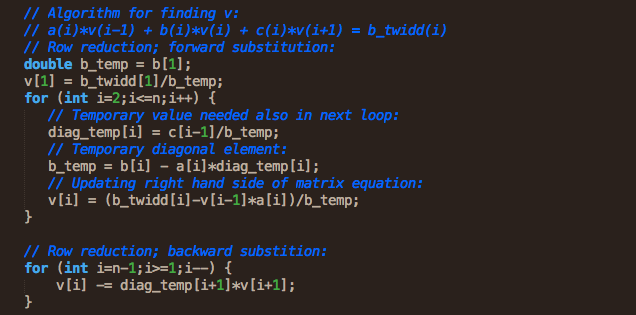
\includegraphics[width = 130mm]{gauss_algoritme.png}\\
  \caption{Figuren viser hvordan forlengs -og baklengs substitusjon kan implementeres i C++. }\label{fig:gausskode}
  \end{center}
\end{figure}
\FloatBarrier

Vi ser at forlengs substitusjons-algoritmen har 6 FLOPS, mens baklengs substitusjon har 2 FLOPS. Vi ender altså opp med at 
\begin{equation}
N_{general} = O(8n)
\end{equation}

\textbf{Spesialtilfelle}\\
I vårt tilfelle har elementene langs de tre diagonalene identisk verdi. Det vil si; alle elementene $a_i$ = $c_i$ = -1, og alle elementene langs diagonalen $b_i$ = 2. Setter vi disse tallene inn i algoritmen vår, får vi for forlengs substitusjon at
\begin{equation}
\tilde{d_i} = 2 - \frac{1}{\tilde{d_i}} = \frac{i+1}{i} \quad \textrm{og} \quad \tilde{e_i} = \frac{\tilde{b_i} + \tilde{e}_{i-1}}{\tilde{d_{i-1}}}
\end{equation}

når $i$ = 2, 3, ..., $n$, mens baklengs substitusjon forenkles til
\begin{equation}
v_i = \tilde{e_i} + \frac{v_{i+1}}{\tilde{d_i}}
\end{equation}

når $i$ = n-1, n-2, ..., 1. Figur \ref{fig:simplified} viser hvordan denne forenklede algoritmen kan implementeres i C++.

\FloatBarrier
\begin{figure}[!ht]
  \begin{center}
  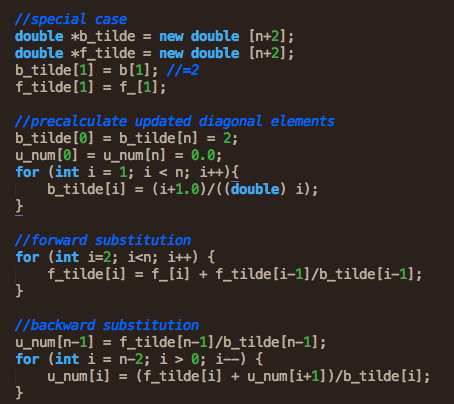
\includegraphics[width = 100mm]{simplified.png}\\
  \caption{Forlengs -og baklengs substitusjon når matrisen har identiske elementer langs diagonalen, over diagonalen og under diagonalen.}\label{fig:simplified}
  \end{center}
\end{figure}
\FloatBarrier

Vi ser nå at antall FLOPS har blitt redusert til 6, slik at 
\begin{equation}
N_{special} = O(6n)
\end{equation}


\subsection{LU-faktorisering}
Det finnes en annen måte å løse det lineære ligningssettet vårt på. En matrise $A \in \Re^{nxn}$ kan LU-faktoriseres dersom dens determinant ikke er lik null. Dersom denne LU-faktoriseringen eksisterer, og $A$ er ikke-singulær (det vi si; kvadratisk og med determinant $\not=$ 0), så er dette en \textit{unik} LU-faktorisering for $A$. Determinanten kan da gis ved
\begin{equation}
det\{\textbf{A}\} = det\{\textbf{LU}\} = det\{\textbf{L}\}det\{\textbf{U}\} = u_{11}u_{22}...u_{nn}
\end{equation}

Siden disse kriteriene er oppfylt for vår matrise $A$, så eksisterer det en unik LU-dekomposisjon for $A$. Det betyr at matrisen $A$ i ligningen $A\textbf{v}=\tilde{\textbf{b}}$ kan dekomponeres til et produkt av to matriser, nemlig $L$ og $U$, hvor $L$ er en nedre triangulær matrise og $U$ er en øvre triangulær matrise: $A=LU$

\begin{equation}
 A = \left(\begin{array}{cccccc}
                          1 & 0 & 0 &\dots    & 0 \\
                           l_{21} & 1 & 0 &\dots &0 \\
                           l_{31} & l_{32} & 1 & \dots &0 \\
                          \vdots  & \vdots   &    &\vdots   \\
                           l_{n1 }& l_{n2}  & l_{n3}  &\dots  &1 \\                         
                      \end{array} \right) 
                      \left(\begin{array}{cccccc}
                          u_{11} & u_{12} & u_{13} &\dots  & u_{1n} \\
                           0 & u_{22} & u_{23} &\dots & u_{2n} \\
                           0 & 0 & u_{33} & \dots & u_{3n} \\
                          \vdots  & \vdots   &    &\vdots   \\
                           0 & 0   & 0  &\dots  & u_{nn} \\                         
                      \end{array} \right)
\end{equation}


LU-faktorisering er en vanlig måte å løse ligningssett på numerisk. For eksempel kan ligningssettet
\[a_{11}x_1 + a_{12}x_2 + a_{13}x_3 + a_{14}x_4 = w_1\]
\[a_{21}x_1 + a_{22}x_2 + a_{23}x_3 + a_{24}x_4 = w_2\]
\[a_{31}x_1 + a_{32}x_2 + a_{33}x_3 + a_{34}x_4 = w_3\]
\[a_{41}x_1 + a_{42}x_2 + a_{43}x_3 + a_{44}x_4 = w_4\]

skrives som en matriseligning på formen

\[\textbf{Ax = w}\]

hvor $A$ og $w$ er kjente størrelser mens $x$ er den ukjente. Ved å bruke LU-faktorisering kan vi skrive

\[\textbf{Ax} \equiv \textbf{LUx = w}\]

Denne ligningen kan splittes i to;
\[\textbf{Ly = w}; \quad \textrm{og} \quad \textbf{Ux = y} \]

Determinanten til $L$ vil være lik 1, siden alle elementene på denne triangulære matrisen har verdien 1. Det betyr at $L$ er en invertibel matrise, slik at vi kan bruke
\[\textbf{Ux} = \textbf{L}^{-1} \textbf{w = y} \]

slik at 
\[\textbf{L}^{-1} \textbf{w = y} \]

Dersom vi finner $\textbf{y}$ først, kan vi finne $\textbf{x}$ ved ligningen $\textbf{Ux = y}$. For en 4x4-matrise vil ligningene komme på formen

 \hfill $y_1 = w_1$
 
 \hfill $l_{21}y_1+ y_2 = w_2$
 
 \hfill $l_{31}y_1 + l_{32}y_2 + y_3 = w_3$
 
 \hfill $l_{41}y_1 + l_{42}y_2 + l_{43}y_3 + y_4 = w_4$
 
 og
 
\hfill $u_{11}x_1 + u_{12}x_2 + u_{13}x_3 + u_{14}x_4 = y_1$
 
\hfill $u_{22}x_2 + u_{23}x_3 + u_{24}x_4 = y_2$

\hfill $u_{33}x_3 + u_{34}x_4 = y_3$

\hfill $u_{44}x_4 = y_4$

\hfill \break

Vi kan nå overføre dette til vår problemstilling. Dersom vi setter inn at $A=LU$ i ligningen $A\textbf{v}=\tilde{\textbf{b}}$, slik at $L(U\textbf{v}) = \tilde{\textbf{b}}$, ender vi opp med to ligningssett:
\begin{equation}
L\textbf{y} = \tilde{\textbf{b}} \quad \textrm{og} \quad U\textbf{v} = \textbf{y}
\end{equation}

Her finner vi først $\textbf{y}$, for så å bruke $\textbf{y}$ til å finne løsningen $\textbf{v}$. Bibliotekene $\texttt{lib.h}$ og $\texttt{lib.cpp}$ inneholder funksjonene vi trenger for å utføre LU-dekomposisjonen. Funksjonen $\texttt{ludcmp}$ finner selve LU-dekomposisjonen, mens $\texttt{lubksb}$ utfører en baklengs substitusjon for å finne løsningen $\textbf{v}$. Firgur \ref{fig:LU} viser hvordan dette kan implementeres i C++:

\FloatBarrier
\begin{figure}[!ht]
  \begin{center}
  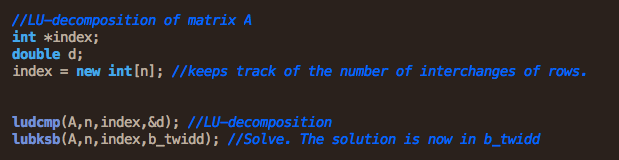
\includegraphics[width = 130mm]{LU.png}\\
  \caption{LU-faktorisering ved bruk av funksjonene $\texttt{lubdcmp}$ og $\texttt{lubksb}$, hentet fra biblioteket $\texttt{lib.cpp}$.}\label{fig:LU}
  \end{center}
\end{figure}
\FloatBarrier

Vi vet at denne algoritmen krever
\begin{equation}
N_{LU} = \frac{2}{3}n^3 + 2n^2 = O(\frac{2}{3}n^3)
\end{equation}

antall FLOPS. Sammenligner vi dette med algoritmene fra forrige seksjon, ser vi at LU-faktorisering faktisk er mer krevende for maskinen.


\section{Resultater}

Figur \ref{fig:n10}, \ref{fig:n100} og \ref{fig:n1000} viser plot av den analytiske løsningen av differensialligningen sammen med den numeriske løsningen vi fant ved hjelp av Gauss-eliminasjon. Det er den generelle algoritmen som er brukt (skrevet i C++), mens et python program tar seg av plottingen. Resultatene er plottet for $n=10$, $n=100$ og $n=1000$.

\FloatBarrier
\begin{figure}[!ht]
  \begin{center}
  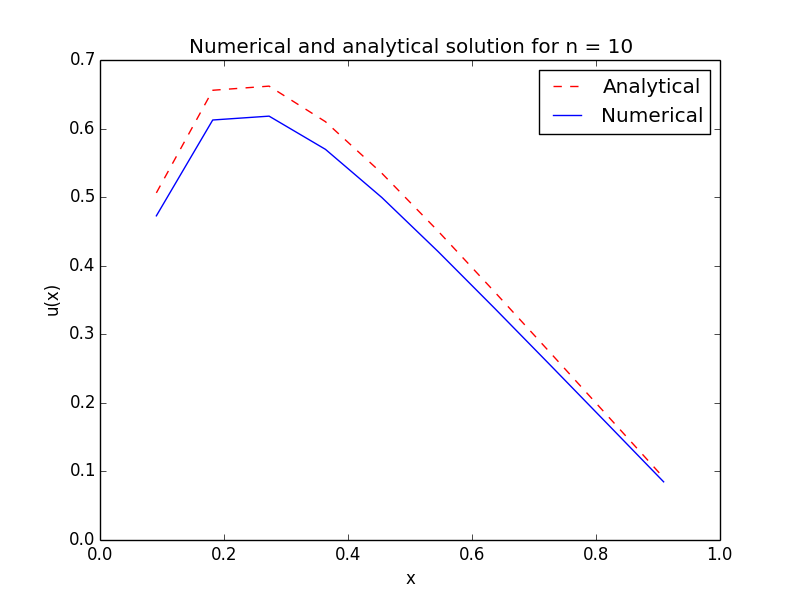
\includegraphics[width = 100mm]{b_n10.png}\\
  \caption{Analytisk og numerisk løsning for $n=10$.}\label{fig:n10}
  \end{center}
\end{figure}
\FloatBarrier

\FloatBarrier
\begin{figure}[!ht]
  \begin{center}
  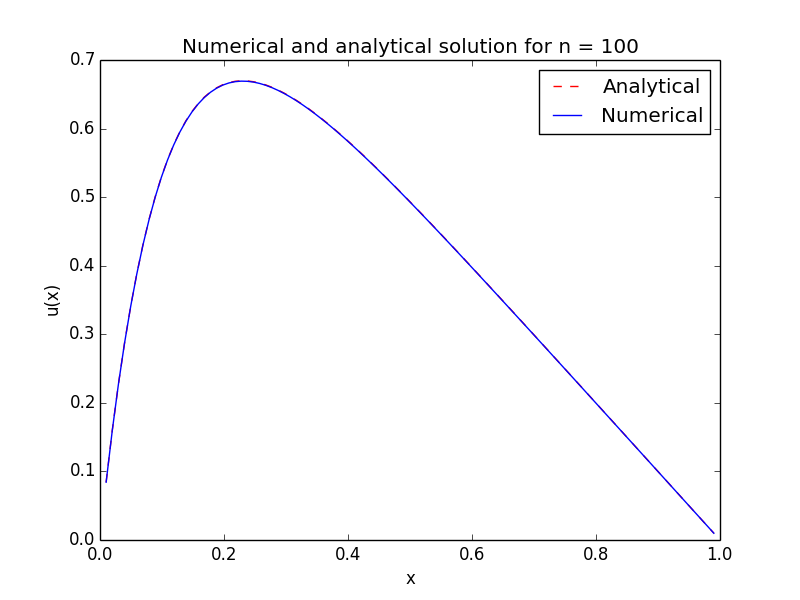
\includegraphics[width = 100mm]{b_n100.png}\\
  \caption{Analytisk og numerisk løsning for $n=100$.}\label{fig:n100}
  \end{center}
\end{figure}
\FloatBarrier

\FloatBarrier
\begin{figure}[!ht]
  \begin{center}
  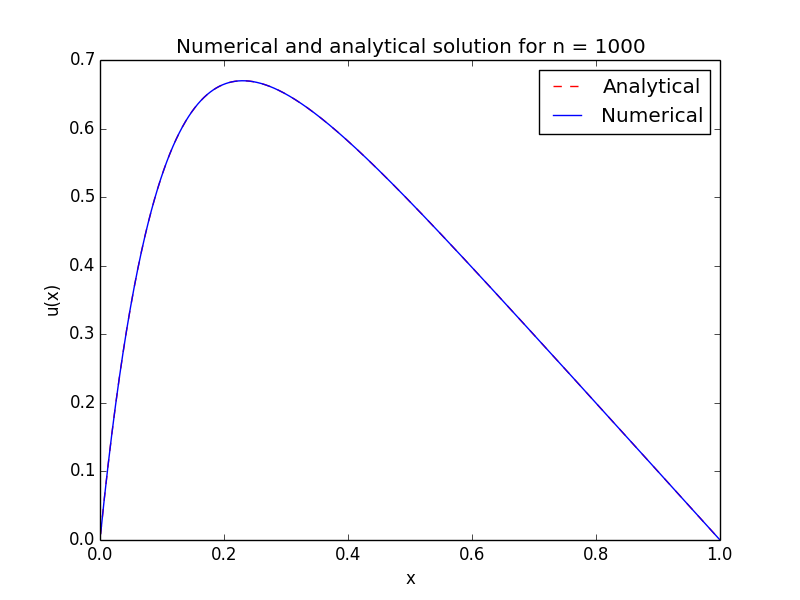
\includegraphics[width = 100mm]{b_n1000.png}\\
  \caption{Analytisk og numerisk løsning for $n=1000$.}\label{fig:n1000}
  \end{center}
\end{figure}
\FloatBarrier

For å finne algoritmens CPU (Central Processing Unit), brukte vi koden gitt i figur \ref{fig:CPU}.

\FloatBarrier
\begin{figure}[!ht]
  \begin{center}
  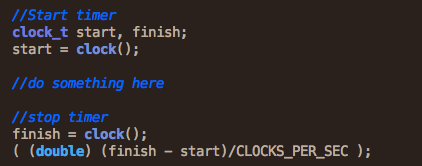
\includegraphics[width = 100mm]{timer.png}\\
  \caption{Metode for å finne et programs CPU.}\label{fig:CPU}
  \end{center}
\end{figure}
\FloatBarrier

Siden det nå er utviklet to algrotimer for å løse samme problemstilling, kan det være interessant å sammenligne disse algoritmenes CPU tid. Vi har sammenlignet CPU tiden mellom den generelle og den spesielle algoritmen for matriser med størrelse opp til $n=10^7$ grid points. Resultatet vises i tabell \ref{CPUgauss}.

\FloatBarrier
\begin{table}[!ht]
\caption{Sammenligning av CPU-tid for de ulike algoritmene}
\centering
\label{CPUgauss}
\begin{tabular}{|c|c|c|}
\hline
$\textbf{n}$      &  $\textbf{Generell CPU [s]}$ & $\textbf{Spesiell CPU [s]}$ \\ 
\hline
$10$     & 2.0000000E-06                  & 3.0000000E-06                  \\ 
\hline
$10^2$ & 8.0000000E-06                  & 5.0000000E-06                  \\ 
\hline
$10^3$ & 4.6000000E-05                  & 4.6000000E-05                  \\ 
\hline
$10^4$ & 0.00038200000                  & 3.1000000E-05                  \\ 
\hline
$10^5$ & 0.0040140000                   & 0.00030400000                   \\ 
\hline
$10^6$ & 0.034464000                    &  0.0032440000          \\ 
\hline       
$10^7$ &  0.37009800                      & 0.031006000     \\
\hline
\end{tabular}
\end{table}
\FloatBarrier


Vi kan også finne størrelsen på den relative feilen i beregningene vi nå har gjort, ved å implementere formelen 
\begin{equation}
\epsilon_i = log_{10} \left(\left| \frac{v_i - u_i}{u_i} \right| \right)
\end{equation} \\

hvor $i = 1, 2, ..., n$. $\epsilon_i$ er en funksjon av $log_{10}(h)$, siden verdiene $v_i$ og $u_i$ avhenger av steglengden $h$. Vi finner den maksimale relative feilen for ulike verdier av $n$ ved å kjøre programmet $\textit{error.cpp}$, med input-verdiene "n" = 10, "number of steps" = 7 og "step increase" = 10. På denne måten loopet programmet gjennom 7 ganger, og kalkulerte den relative feilen med en økning på x10 for hver gang, helt opp til $n = 10^7$. Tabell \ref{error} viser resultatene.   

\FloatBarrier
\begin{table}[!ht]
\caption{Relativ feil i den generelle algoritmen}
\centering
\label{error}
\begin{tabular}{|c|c|c|}
\hline
$\textbf{n}$   &  $\textbf{log}_{10}(h)$  & $\textbf{log}_{10}(\epsilon_{max})$ \\
\hline
$10$     & -1.0413927  &   -1.3589135                  \\ 
\hline
$10^2$ & -2.0043214   &  -3.2621439                 \\ 
\hline
$10^3$ & -3.0004341  &   -5.2541384               \\ 
\hline
$10^4$ & -4.0000434   &  -7.2533984                  \\ 
\hline
$10^5$ & -5.0000043    &  -9.0436161                \\ 
\hline
$10^6$ & -6.0000004   &   -6.3508347         \\ 
\hline       
$10^7$ & -7.0000000   &   -6.1988961      \\
\hline
\end{tabular}
\end{table}
\FloatBarrier

Til slutt sammenlignes CPU-tiden mellom en standard LU-faktorisering og den generelle tridiagonale algoritmen. Dette ble gjort for $n=10$, $n=100$ og $n=1000$. Resultatene er vist i tabell \ref{LUCPU}.

\FloatBarrier
\begin{table}[!ht]
\caption{CPU-tiden til LU-faktoriseringen og den generelle tridiagonale løsningen.}
\centering
\label{LUCPU}
\begin{tabular}{|c|c|c|}
\hline
$\textbf{n}$   &  $\textbf{CPU [s]: LU}$  & $\textbf{CPU [s]: Tridiagonal}$ \\
\hline
$10$     & 0.00013400000  &   1.0000000E-06                  \\ 
\hline
$100$ & 0.0018050000   &  5.0000000E-06                 \\ 
\hline
$1000$ & 2.8918500     &   3.4000000E-05               \\ 
\hline
\end{tabular}
\end{table}
\FloatBarrier



\section{Diskusjon}
Vi ser av figurene \ref{fig:n10}, \ref{fig:n100} og \ref{fig:n1000} at den implementerte algortimen for en generell tridiagonal matrise fungerer. Som forventet vil den numeriske løsningen nærme seg den analytiske løsningen jo større $n$ er. Dette ses særlig godt dersom man sammenligner figur \ref{fig:n10} med de to andre figurene. \\

I tabell \ref{error} ser vi at den maksimale relative feilen minker jo større $n$ blir. Et sted i mellom $n=10^5$ og $n=10^6$ vil den maksimale relative feilen begynne å øke igjen, dette kommer av at steglengden $h$ har blitt så liten at vi ender opp med avrundingsfeil. Man vil altså ikke få noen mer nøyaktig numerisk løsning enn ved $n=10^5$.\\

Vi endte opp med to ulike algortimer som utførte samme jobb; en generell og en spesiell. Den generelle algoritmen kan brukes på en vilkårlig tridiagonal matrise, mens den spesielle algoritmen er en (forenklet) versjon av denne hvor vi har identiske tall langs diagonalen og i diagonalen over og under hoveddiagonalen. Den generelle algoritmen endte opp med antall FLOPS på $O(8n)$, mens den spesielle hadde $O(6n)$ FLOPS. Det vil da være rimelig å anta at den spesielle algoritmen vil ha (noe) kortere CPU tid enn den generelle. Ser vi nærmere på tabell \ref{fig:CPU}, ser vi at dette stemmer. Det skal likevel nevnes at dette ikke var noen banebrytende forskjell i CPU tid. Forskjellen blir mer markant for store $n$-verdier. \\

Når det kommer til LU-faktoriseringen, ser vi tydelig forskjell når det kommer til CPU (se tabell \ref{LUCPU}). Det har tidligere blitt nevnt at algoritmen for den generelle tridiagonale matrisen krever $O(8n)$ FLOPS, mens LU-fatoriseringen krever $O(\frac{2}{3}n^3)$ FLOPS. Når $n$ blir stor kan vi derfor forvente at CPU tiden vil øke lineært som funksjon av $n$ for den tridiagonale løsningsmetoden, mens LU-faktoriseringen vil øke kubisk.\\

Siden vi i vårt tilfelle har med en tridiagonal matrise å gjøre, vil en LU-faktorisering bruke unødig antall FLOPS, for ikke å snakke om minne i datamaskinen til å lagre alle matriseelementene. Når $n$ blir betraktelig stor (størrelsesorden $10^4$ og oppover), vil vi ende opp med en gigantisk matrise. Dersom vi hadde valgt $n=10^5$, ville vi endt opp med en matrise med $10^5\cdot 10^5 = 10^{10}$ elementer! Alle disse elementene bruker en viss menge lagringsplass. Dersom hvert element er av typen "double" ville vi trengt 8byte$\cdot10^{10} = 80GB$ med lagringsplass!


\section{Konklusjon}
Siden vi i vårt tilfelle hadde et ligningssett som førte til en tridiagonal matrise, sier det seg selv at det vil være unødig å anvende vanlig Gauss-elinimasjon eller standard LU-dekomposisjon, med tanke på antall FLOPS. Det egnet seg derimot å anvende en egen utviklet algoritme beregnet på tridiagonale matriser!\\

Vi har i dette prosjektet sett at vi kan løse en én dimensjonal Poisson-ligning numerisk på flere ulike metoder. Metodene varierer i antall FLOPS og beregningstid. Vi startet med å anvende Gauss-eliminasjon på en generell matrise, og fant ut at denne metoden kunne forenkles siden matrisen var tridiagonal. Vi kunne da se bort fra alle null-elementene og heller lagre de tre diagonalene i form av vektorer. Dette ga oss et antall FLOPS på formen $O(8n)$. Vi kalkulerte så den maksimale relative feilen i den numeriske løsningen ved å sammenligne med den gitte analytiske løsningen, og fant at vi hadde minst relativ feil når $n=10^5$. \\

Den andre metoden vi brukte var LU-faktorisering. Dette er en standard metode å løse ligningssett på. Ulempen med denne metoden er at den allokerer plass i minnet til hvert eneste element i matrisen, slik at for store $n$-verdier vil dette være en tidkrevende metode. I vårt tilfelle var ikke dette den optimale metoden, siden matrisen vår var tridiagonal.


\section{Vedlegg}
Alle koder og resultater som er brukt i rapporten finnes på Github-adressen: https://github.com/livewj/Project-1



\bibliography{Referanser}
\begin{thebibliography}{9}

\bibitem{squires}
  Kursets offisielle Github-side $\textit{FYS3150 - Computational Physics}$
  https://github.com/CompPhysics/ComputationalPhysics,
  03.09.2016  
  
\bibitem{}
  Slides fra kursets offisielle nettside: "Matrices and linear algebra" http://compphysics.github.io/ComputationalPhysics/doc/web/course, 14.09.16
  
\bibitem{}
 https://no.wikipedia.org/wiki/CPU, 16.09.16
    
\end{thebibliography}

\end{document}

